\documentclass[border=4pt]{standalone}
\usepackage[utf8]{inputenc}\usepackage[T1]{fontenc}\usepackage{mathptmx}
\usepackage{tikz}\usetikzlibrary{positioning,arrows.meta,calc}
\begin{document}
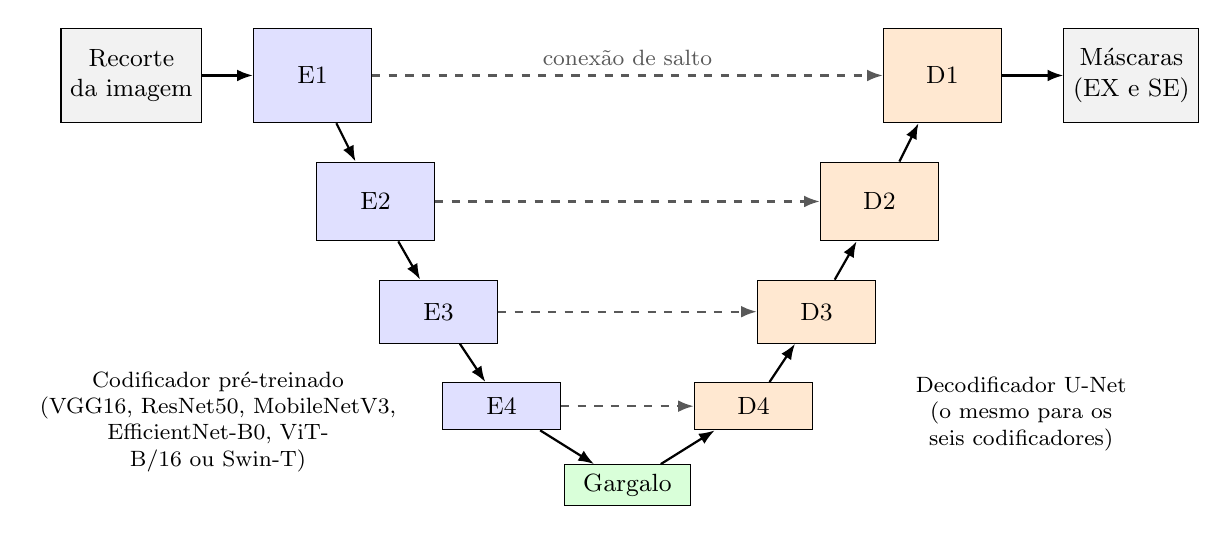
\begin{tikzpicture}[font=\small,
  enc/.style={draw,fill=blue!12,minimum width=1.5cm,align=center},
  dec/.style={draw,fill=orange!18,minimum width=1.5cm,align=center},
  arr/.style={-{Latex[length=2mm]},thick},
  skip/.style={-{Latex[length=2mm]},thick,dashed,gray!70!black}]
\node[draw,fill=gray!10,align=center,minimum height=1.2cm] (in) at (-2.3,0) {Recorte\\da imagem};
\node[enc,minimum height=1.2cm] (e1) at (0,0) {E1};
\node[enc,minimum height=1.0cm] (e2) at (0.8,-1.6) {E2};
\node[enc,minimum height=0.8cm] (e3) at (1.6,-3.0) {E3};
\node[enc,minimum height=0.6cm] (e4) at (2.4,-4.2) {E4};
\node[draw,fill=green!15,minimum width=1.6cm,minimum height=0.5cm] (b) at (4.0,-5.2) {Gargalo};
\node[dec,minimum height=0.6cm] (d4) at (5.6,-4.2) {D4};
\node[dec,minimum height=0.8cm] (d3) at (6.4,-3.0) {D3};
\node[dec,minimum height=1.0cm] (d2) at (7.2,-1.6) {D2};
\node[dec,minimum height=1.2cm] (d1) at (8.0,0) {D1};
\node[draw,fill=gray!10,align=center,minimum height=1.2cm] (out) at (10.4,0) {Máscaras\\(EX e SE)};
\draw[arr] (in) -- (e1);
\draw[arr] (e1) -- (e2); \draw[arr] (e2) -- (e3); \draw[arr] (e3) -- (e4); \draw[arr] (e4) -- (b);
\draw[arr] (b) -- (d4); \draw[arr] (d4) -- (d3); \draw[arr] (d3) -- (d2); \draw[arr] (d2) -- (d1);
\draw[arr] (d1) -- (out);
\draw[skip] (e1) -- node[above,font=\footnotesize]{conexão de salto} (d1);
\draw[skip] (e2) -- (d2); \draw[skip] (e3) -- (d3); \draw[skip] (e4) -- (d4);
\node[align=center,font=\footnotesize,text width=4.6cm] at (-1.2,-4.4) {Codificador pré-treinado\\(VGG16, ResNet50, MobileNetV3,\\EfficientNet-B0, ViT-B/16 ou Swin-T)};
\node[align=center,font=\footnotesize,text width=3.6cm] at (9.0,-4.3) {Decodificador U-Net\\(o mesmo para os\\seis codificadores)};
\end{tikzpicture}
\end{document}
